\title{Entrevista}
\subtitle{com Ricardo Bergamo Schenato}
\maketitle
\begin{wrapfigure}{l}{0.15\textwidth}
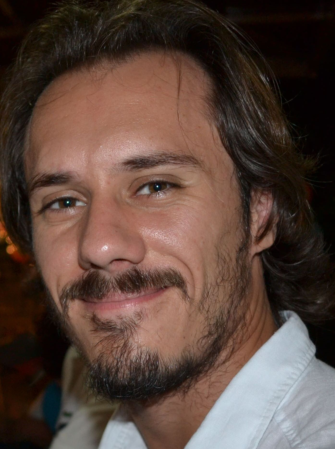
\includegraphics[width=0.15\textwidth]{figuras/foto-ricardo}
\end{wrapfigure}








Nesta edição de \pedometria, entrevistamos o Professor Doutor Ricardo Bergamo Schenato para falar um pouco sobre a Pedometria e a Modelagem Ambiental, suas potencialidades, dificuldades e perspectivas futuras no Brasil. O Dr. Ricardo atualmente é docente no Departamento de Solos - Setor de Gênese, Morfologia e Classificação de Solos da Universidade Federal de Santa Maria (UFSM). Sua formação pós ensino médio foi realizada na UFSM, onde cursou Agronomia e o mestrado em Ciência do Solo na área de Química do solo. Fez doutorado em Ciência do solo na Universidade Federal do Rio Grande do Sul (UFRGS). Sua tese contemplou temas relacionados a modelagem e fluxos de gases de efeito estufa no Estado do RS.
\\
\textbf{Pedometria} - O que levou você a se interessar e estudar temas relacionados a modelagem ambiental e em especial propriedades do solo?\\
\\
\textbf{Ricardo} - Na iniciação científica meu primeiro contato com a espacialização de propriedades e atributos de solo ocorreu quando trabalhei com a temática de agricultura de precisão, onde experimentei todas as fases da pesquisa. Nesta época comecei a interessar-me nas questões ambientais que envolviam o solo por ocasião da leitura de textos sobre qualidade do solo e por constatar que a maioria da pesquisa estava focada na melhoria ou conservação da capacidade produtiva em detrimento de uma compreensão global do sistema. Ainda na graduação, o interesse crescente na otimização dos recursos empregados na produção primária determinaram a escolha por estudar a transferência de elementos na paisagem, tornando-se o objeto de minha dissertação de mestrado. O interesse pela modelagem, em um sentido amplo, deveu-se às potencialidade que suas ferramentas oferecem para a pesquisa ambiental, podendo-se citar a capacidade de simular condições pretéritas e futuras, avaliar variáveis que seriam de difícil mensuração a campo, elaborar cenários complexos, extrapolar resultados no tempo e no espaço, auxiliar no planejamento da pesquisa empírica, entre outros.\\
\\
\textbf{Pedometria} - Quais são os projetos de pesquisa que você está desenvolvendo relacionados a modelagem ambiental e espacialização de propriedades do solos?\\
\\
\textbf{Ricardo} - Em novembro de 2013 ingressei como docente da UFSM, portanto, devido à entrada recente, estou readequando minhas linhas de pesquisa com o intuito de colaborar mais eficientemente com os pesquisadores do Departamento de Solos. A Pedometria será a principal linha de pesquisa, especialmente como subsídio ao Mapeamento Digital do Solo (MDS). O foco inicial será na avaliação de técnicas para determinar a distribuição espacial de classes e atributos do solo. A abrangência das aplicações da Pedometria, aliada ao caráter incipiente desta área quando comparada a outras da Ciência do Solo, resultam em uma grande possibilidade de interação, de tal forma que projetos com outras áreas do conhecimento certamente serão desenvolvidos. Além disso, pretendo dar continuidade e ampliar a pesquisa que desenvolvi na minha tese \citep{Schenato:2013}, visando a modelagem dos ciclos de C e N no solo e seu efeito na emissão de gases de efeito estufa, bem como implementar a espacialização dos resultados já obtidos. O objetivo principal desta linha é estimar os impactos, positivos e negativos, da atividade agropecuária e auxiliar no uso racional dos recursos.\\
\\
\textbf{Pedometria} - Qual sua opinião a respeito do cenário atual sobre as pesquisas em modelagem ambiental e predição de propriedades do solo no Brasil?\\
\\
\textbf{Ricardo} - A adesão dos pesquisadores em solos brasileiros a estes temas é relativamente recente, tanto que grande parte da produção científica nacional está concentrada especialmente na última década. Esta observação também mostra que existe um número crescente de profissionais publicando em ambos os assuntos, refletindo a importância destes e indicando um fortalecimento dos grupos de pesquisa. Os custos baixos e a facilidade de obtenção de dados de sensores remotos são fatores que propiciaram o aumento da sua utilização para a determinação de atributos do terreno como declividade, elevação, aspecto, plano de curvatura, radiação solar, índices topográficos, índice de convergência, entre outros, abrindo um campo importante para trabalhos que enfoquem a implicação destes atributos na dinâmica de formação e evolução do solo e da paisagem. A prevalência na utilização tanto da modelagem do terreno como na predição de propriedades do solo está voltada ao MDS, o que pode ser justificado pela lacuna existente no nosso país no tocante ao conhecimento mais detalhado das classes de solo e ao aumento da demanda por informações mais detalhadas como subsídio para aplicações práticas.  O planejamento de projetos agrícolas, a adequação do uso do solo urbano e a implementação de atividades de recuperação ambiental são apenas alguns exemplos que necessitam da definição adequada da classe e/ou de propriedades do solo e estas informações nem sempre estão disponíveis ou a escala não é adequada. Nestes casos a predição de propriedades pode facilitar a obtenção dos dados e baratear o custo dos projetos, considerando que o levantamento e a determinação clássica tendem a ser mais onerosos e demorados. A frequência na aplicação de funções de pedotransferência pelos pesquisadores brasileiros também merece destaque. A abrangência das informações que podem ser geradas e a disseminação do uso dessas funções tem um potencial muito grande, podendo contribuir, por exemplo, na evolução do Sistema Brasileiro de Classificação de Solos, aliando a classificação numérica de dados de solo com a classificação hierárquica. Nesse sentido, a modelagem do terreno e a predição dos atributos do solo certamente contribuirão sobremaneira na determinação dos padrões de distribuição de classes de solo, inclusive com bons resultados já demonstrados em locais com embasamento geológico complexo. Apesar das ferramentas estarem cada vez mais acessíveis, a busca crescente por informações detalhadas, o tamanho do território e a heterogeneidade dos solos brasileiros demandarão muito mais do que já foi realizado e os profissionais deverão estar atentos para fornecer subsídios adequados aos processos de tomada de decisão.\\
\\
\textbf{Pedometria} - Qual a sua opinião a respeito da modelagem espacial de atributos do solo, geoestatística aplicada na ciência do solo, geoprocessamento e linguagem de programação como disciplinas nos cursos de Pós-Graduação da área de solos no Brasil?\\
\\
\textbf{Ricardo} - Esses tópicos são essenciais se desejarmos qualificar e expandir a modelagem nos cursos Pós-Graduação em solos, e poderiam ser apresentados já em nível de graduação, de forma optativa. A falta de oferta de disciplinas que abordem esses assuntos está relacionada, segundo minha opinião, ao baixo número de profissionais aptos a ministrá-las aliado a sobrecarga daqueles capacitados, por já atuarem em outras atividades de ensino, pesquisa, extensão e administração. Um aspecto crítico que deve ser considerado é a deficiência no embasamento matemático da maioria da população universitária, o que representa um desafio adicional a ser superado. A oferta de uma disciplina sobre noções de programação, orientada para problemas práticos, aos alunos de graduação ajudaria a diminuir a resistência dos discentes com a área das exatas, pois permitiria aplicar conhecimentos abstratos na resolução de problemas mais tangíveis e também serviria como uma base útil para quem desejar integrar-se na iniciação científica em qualquer área, não somente em solos.\\
\\
\textbf{Pedometria} - Pela sua experiência na área de modelagem ambiental, quais as principais dificuldades e desafios encontrados para os pesquisadores brasileiros desenvolverem seus trabalhos nessa área?\\
\\
\textbf{Ricardo} - Para mim está claro que a limitação principal é a insuficiência de pessoal qualificado, consequentemente, a formação de profissionais habilitados a trabalhar com modelagem ambiental é o maior desafio. Por ser uma área relativamente nova dentro da Ciência do Solo existem poucas pessoas habilitadas para trabalhar com este campo da modelagem. O rol de habilidades a serem desenvolvidas por quem pretende trabalhar na modelagem ambiental é um obstáculo adicional, pois além de conhecer as características e interações do sistema a ser modelado é necessário ter um conhecimento básico de áreas como Cálculo, Estatística e Programação, por exemplo. A quantidade de dados disponíveis pode ser apontado como mais um fator limitante, uma vez que dados empíricos confiáveis são necessários para o desenvolvimento, calibração e validação de modelos. Naturalmente o volume de dados existente é bastante heterogêneo de uma variável para outra, mas o Brasil, de uma forma geral, ainda tem poucas medições quando comparado com outros países que possuem maior tradição de monitoramento e experimentos de longo prazo e com representatividade territorial. Esta questão é historicamente negligenciada e deveria ser encarada com mais seriedade no nosso país, incentivado a coleta de dados de forma contínua, através de programas de monitoramento, e com uma organização que permita representar adequadamente a complexidade dos ecossistemas brasileiros, fomentando a formação de redes de pesquisa. A estrutura do armazenamento dos dados produzidos também deve ser considerada pelos pesquisadores como uma forma de garantir a segurança dos dados e facilitar o acesso futuro. Os resultados produzidos pelos diversos grupos de pesquisa normalmente são armazenados sem a estrutura de um banco de dados propriamente dito, dificultando a pesquisa eficiente pelos modeladores, além de não ser raro que algumas informações acabem sendo perdidas. Nesse sentido, a estruturação de bancos de dados seria de grande valia para os pesquisadores que desejassem acessar o material produzido, além de facilitar o compartilhamento entre diferentes grupos.\\
\\
\textbf{Pedometria} - Você vê a modelagem ambiental e predição de atributos do solo como ferramentas promissoras para serem utilizadas na obtenção de informações de qualidade sobre solos e assim abastecer banco de dados de solos brasileiros?\\
\\
\textbf{Ricardo} - Sem dúvida nenhuma. Diria até que elas não são somente promissoras, são fundamentais. A demanda por informações de qualidade relativas aos solos brasileiros tem aumentado muito nos últimos anos e diversos grupos vêm trabalhando muito bem para preencher as lacunas existentes. Por outro lado, nosso país tem uma dimensão continental e apresenta uma grande heterogeneidade de solos e condições ambientais, o que nos mostra que ainda há muito trabalho a fazer. Considerando essa situação e levando em conta aspectos logísticos, metodológicos e econômicos, não vejo como as instituições poderão prover essa demanda somente através de medições in loco, ainda que consideremos o médio e longo prazo. Deve-se destacar também o aspecto quantitativo e a capacidade de determinação das incertezas através dos processos de modelagem, o que qualifica a informação gerada e permite uma tomada de decisão mais segura por quem a utiliza. Portanto, a capacidade de interação entre a pesquisa dita tradicional com as técnicas mais recentes de modelagem determinará a qualidade e a velocidade de produção e disponibilização das informações que alimentarão os bancos de dados de solos brasileiros
Sem dúvida a pedometria tem elevado potencial para geração de dados para um banco de dados.\\
\\
\textbf{Pedometria} - Qual a sua opinião a respeito da interdisciplinaridade nos grupos de pesquisa da área de solos para desenvolver trabalhos que contribuam para meio científico? Em sua opinião, existe interdisciplinaridade nos grupos de pesquisa do Brasil? Sim ou Não? Por quê?\\
\\
\textbf{Ricardo} - Na Ciência do Solo há grandes possibilidades - e necessidade - de interação com diversas áreas, como por exemplo, Geologia, Química, Matemática, Estatística, Ciência da Computação, Geomática, entre outras. Existem iniciativas de cooperação bem sucedidas  em diversos grupos de pesquisa brasileiros, no entanto, essa potencialidade poderia ser mais explorada. Praticamente toda a ciência atual é desenvolvida sob a égide do paradigma clássico cartesiano, cujo mito fundacional alicerça-se sobre a ideia de que para conhecer o todo é preciso antes conhecer as partes separadamente, visão que vem sendo superada pela abordagem holística, mais integradora. No entanto, os reflexos da setorização é notado na organização estrutural e na dinâmica de trabalho de muitos grupos de pesquisa, em geral levando-os a fecharem-se para profissionais de outras áreas. É difícil imaginar uma mudança nas estruturas dos grupos de pesquisa, pois passa por mudanças em níveis não gerenciáveis internamente pelo grupos, como por exemplo de caráter institucional. Além disso, o sistema atual tem conseguido bons resultados em termos de produção científica e formação de mão-de-obra qualificada tornando-o mais resistente a mudanças profundas. Outro aspecto que vai ao encontro da necessidade de cooperação entre os pesquisadores, e deve ser considerado, é a grande quantidade e a taxa de geração de novas informações na sociedade atual. A profusão de informação é uma situação nunca antes experimentada, sendo que a sua apropriação e, principalmente, a sua transformação em conhecimento requer o domínio de várias áreas. Considerando este panorama, fica evidente a impossibilidade de um único indivíduo dominar todo o ferramental teórico e prático necessário para a produção científica de qualidade, reforçando a necessidade de interação. A saída da zona de conforto é uma necessidade ao interagir com outras áreas do conhecimento, uma vez que para manter a boa comunicação e troca de informações o pesquisador deve dominar minimamente o conteúdo de uma disciplina com a qual não está familiarizado. A exposição ao erro aumenta quando se resolve incursionar em temas novos e certamente não é uma situação a qual todos estão dispostos a submeter-se. A implementação prática da interdisciplinaridade não é uma tarefa simples, mesmo que seja uma vontade do pesquisador e/ou grupo de pesquisa. Um exemplo é a inserção de graduados em áreas tradicionalmente distantes das absorvidas pelos cursos de Pós-Graduação na área de solos. Se por um lado verifica-se relativamente poucos estudantes nestes cursos com formação diversa das Ciências Rurais por outro devemos considerar o efeito prático de um matemático, por exemplo, com título de Doutor em Ciência do Solo. Quais seriam as possibilidades de inserção deste profissional no mercado de trabalho? O ingresso de profissionais sem nenhuma base em solos em programas de Pós-Graduação nesta área seria a melhor forma de implementar a interdisciplinaridade? Apesar das dificuldades acredito que os esforços no sentido de uma maior interação dentro dos grupos de pesquisa e entre pesquisadores de grupos de pesquisa distintos devem ser encorajados e como consequência pode-se esperar uma  qualidade crescente das pesquisas realizadas e um destaque ainda maior da Ciência do Solo brasileira no cenário internacional.\\
\\
\textbf{Pedometria} - Na sua opinião, qual o interesse do público leitor por temas relacionados a pedometria e modelagem espacial e temporal de informações ambientais?\\
\\
\textbf{Ricardo} - Os leitores dos dois temas citados ficam restritos a quem está envolvido em pesquisas relacionados aos mesmos. A questão a ser respondida é: como despertar o interesse das pessoas, ligadas ou não à pesquisa, pela leitura destes temas? A pedometria e a modelagem espacial não estão sozinhas em um dos pontos que considero mais sensíveis relativos a pesquisa científica brasileira: a divulgação científica. Os leitores que buscam conteúdos científicos, além de estarem ligados a algum projeto de pesquisa, o fazem com bastante seletividade, restringindo-se ao seu tema de investigação. As revistas científicas são a principal fonte de pesquisa nestes casos, mas para propiciar o contato com o público leigo deve-se explorar os diversos canais disponíveis, utilizando uma linguagem adequada, tanto para informar quanto para incentivar a curiosidade sobre diversos temas científicos. Outra questão chave também deve ser respondida: Como podemos despertar o interesse das crianças e jovens pela pesquisa científica, se até o ingresso no ensino superior a maioria nunca teve contato com este assunto? No ensino básico e fundamental encontram-se oportunidades ímpares para promover o primeiro contato com a ciência. As escolas têm fomentado as feiras de ciência, o que é excelente quando a execução é adequada, ou seja, quando os alunos realmente são incentivados a pensar e executar o seu projeto. Mas muito mais pode ser realizado, como por exemplo a inserção de noções de solos nas disciplinas do currículo escolar. Atualmente as crianças têm contato cada vez mais cedo com dispositivos eletrônicos e as escolas estão sendo equipadas paulatinamente, então há um potencial incrível para ser explorado. O interesse dos alunos certamente seria maior se pudessem, por exemplo, utilizar um software de fácil utilização, e até lúdico, onde fosse possível manipular as características da paisagem e observar o resultado do efeito da vegetação, da inclinação e comprimento das encostas, entre outros, sobre a dinâmica da água. Disciplinas como Geografia, Matemática, Biologia e Física poderiam explorar a experiência neste tipo de ferramenta para o ensino dos respectivos conteúdos.








\begin{footnotesize}
\begin{thebibliography}{99}
\bibitem[Schenato(2013) Schenato]{Schenato:2013}
R.B. Schenato (2013)
\newblock Simulação de fluxos de gases de efeito estufa em sistemas de manejo do solo no sul do Brasil.
\newblock {\em Tese de doutorado, Universidade Federal do Rio Grande do Sul}, 126p.
\end{thebibliography}
\end{footnotesize}








\address{Jean Michel Moura-Bueno\\
\footnotesize
Universidade Federal de Santa Maria\\
\email{bueno.jean1@gmail.com}}
%%% Local Variables:
%%% mode: latex
%%% TeX-master: 3rd-edition.tex
%%% End:
